\documentclass[10pt,twocolumn,a4paper]{article}


% Use Times-like font for pdfLaTeX
\usepackage{mathptmx}

% Set up page geometry
\usepackage[a4paper, margin=1in]{geometry}
\usepackage[utf8]{inputenc}
\usepackage[T1]{fontenc}
\usepackage[german]{babel} % Use 'english' for English text
\usepackage{amsmath}
\usepackage{graphicx}
\usepackage{geometry}
\usepackage{booktabs} % For professional tables
\usepackage{hyperref}
\usepackage{parskip} % Space between paragraphs
\usepackage[backend=biber]{biblatex}
\addbibresource{references.bib} % BibTeX file for references

% Header and footer
\usepackage{fancyhdr}
\pagestyle{fancy}
\fancyhead[L]{Spektroskopie}
\fancyhead[C]{Digitale Holographische Spektroskopie}
\fancyhead[R]{Lorenz Saalmann}
\fancyfoot[C]{\thepage}

\begin{document}

\setlength{\parindent}{0pt}

% Document starts here

\begin{titlepage}
    \centering
    \begin{figure}
        \centering
        
\includegraphics[width=0.3\textwidth]{images/jlu_logo.jpeg}
    \end{figure}
    \vspace*{2cm}
    \text{Ausarbeitung} \\
    \Large{Digitale Holographische Spektroskopie} \\
    \vspace{2cm}
    \normalsize{Lorenz Saalmann (8104072)} \\
    \vfill
    \normalsize{{Spektroskopie, SS 25}} \\
    \small{PD Dr. Arash Rahimi-Iman, Dipl.-Ing.} \\
\end{titlepage}

\newpage

\section{Einführung}
\vspace{-0.3cm}
\hspace{.0cm}\fontsize{9}{0}{\bf{KI-unterstützt von GPT-3.5 \cite{AI}}}
\vspace{0.4cm}
\\
\small
Spektroskopie befasst sich mit der Wechselwirkung von Licht und Materie. Im Fokus steht dabei die Abhängigkeit der Lichtintensität von Wellenlänge oder Frequenz. Damit lassen sich Phänomene wie Absorption, Emission und Streuung untersuchen. Da die beschriebene Wechselwirkung so grundlegend ist, findet die Spektroskopie in sehr vielen Bereichen Anwendung, wie zum Beispiel in der Chemie, Physik, Astronomie und Biologie. Sie dient der Materialanalyse, Zusammensetzungsbestimmung und der Untersuchung von physikalischen Eigenschaften von Stoffen. Konventionelle spektroskopische Verfahren basieren meist auf Intensitätsmessungen und liefern dadurch indirekte Informationen über Struktur oder Zusammensetzung eines Objekts. Insbesondere die Phaseninformation -- und damit quantitative Aussagen zur optischen Weglänge oder Topographie -- bleiben dabei unzugänglich.

Im Gegensatz dazu ermöglicht Holographie eine vollständige Erfassung des komplexen Lichtfeldes (Amplitude und Phase), wodurch eine hochauflösende dreidimensionale Rekonstruktion von Objekten möglich wird. Digitale Holographie überträgt dieses Prinzip in den digitalen Bereich: Mit modernen Bildsensoren und numerischen Rekonstruktionsverfahren lässt sich das holographisch aufgezeichnete Interferenzmuster analysieren. Kombiniert mit spektralen Messmethoden entsteht so die Digitale Holographische Spektroskopie (DHS). So können phasen-sensitive, räumliche und spektrale Informationen gleichzeitig erfasst werden, was eine tiefe Analyse des Lichtfeldes ermöglicht. Besonders in der Nanophotonik, der biomedizinischen Bildgebung und der Untersuchung optischer Materialien bietet DHS entscheidende Vorteile.

\section{Grundlagen der Holographie}
Ähnlich wie bei Photographie, ist das Ziel der Holographie, ein Objekt abzubilden. Der entscheidende Unterschied ist, dass dabei nicht nur die Intensität des Lichts an jedem Punkt auf einem Film erfasst, sondern auch dessen Phase. Dadurch bleibt die Tiefeninformation des Lichtfeldes erhalten und es ist möglich das Lichtfeld des Objekts sehr genau zu reproduzieren. Entdeckt wurde die Holographie von Dénes Gábor, einem ungarischen Ingenieur, 1947. Entscheidend für die Aufnahme dieser Informationen ist Interferenz. Eine monochromatische, kohärente Lichtquelle wird genutzt und in einen Referenzstrahl und einen Objektstrahl aufgeteilt. Bei einem Transmissionshologramm fällt die Referenz schräg auf den Film und interferiert mit dem Objektstrahl, nachdem dieser vom Objekt reflektiert wurde. So ist die Information über die Entfernung zum Objekt in dem Interferenzmuster in jedem Punkt erhalten, wobei die Auflösung des Films begrenzend wirkt. Um ein physisches Transmissionshologramm darzustellen, wird das auf Film aufgenommene Interferenzmuster nur mit dem Referenzstrahl beleuchtet. Das Muster wirkt dann als Beugungsgitter und das hinter dem Gitter resultierende Lichtfeld enthält das des Objektstrahls \cite{Gabor}.

Beim Betrachten ist ein virtuelles Bild des Objekts sichtbar, was beidäugig den vollständigen dreidimensionalen Eindruck des Objekts gibt. Teilt man den Film, kann durch beide Teile das gesamte Bild unter dem richtigen Winkel gesehen werden. Das gibt einen Hinweis darauf, dass Hologramme eine große Menge an Informationen speichern können.

Die Intensität des überlagerten Feldes kann als das Betragsquadrat der komplexen Wellen $R$ und $O$ beschrieben werden:
\begin{equation}
    |R + O|^2 = |R|^2 + |O|^2 + R^* O + R O^*.
\end{equation}
So kann das Interferenzmuster auf dem Film beschrieben werden. Wird dieses nun zur Rekonstruktion mit der Referenz $R$ beleuchtet ergibt sich:
\begin{equation}
    R(|R|^2 + |O|^2 + R^* O + R O^*) = R(|R|^2 + |O|^2) + |R|^2O + |R|^2O*.
\end{equation}
Hier kann man erkennen, dass die Objektwelle $O$ und ihr konjugiert komplexes $O*$ um $|R|^2$ skaliert, sowie eine mit eine multiplizierte Referenzwelle.

\begin{figure}
    \centering
    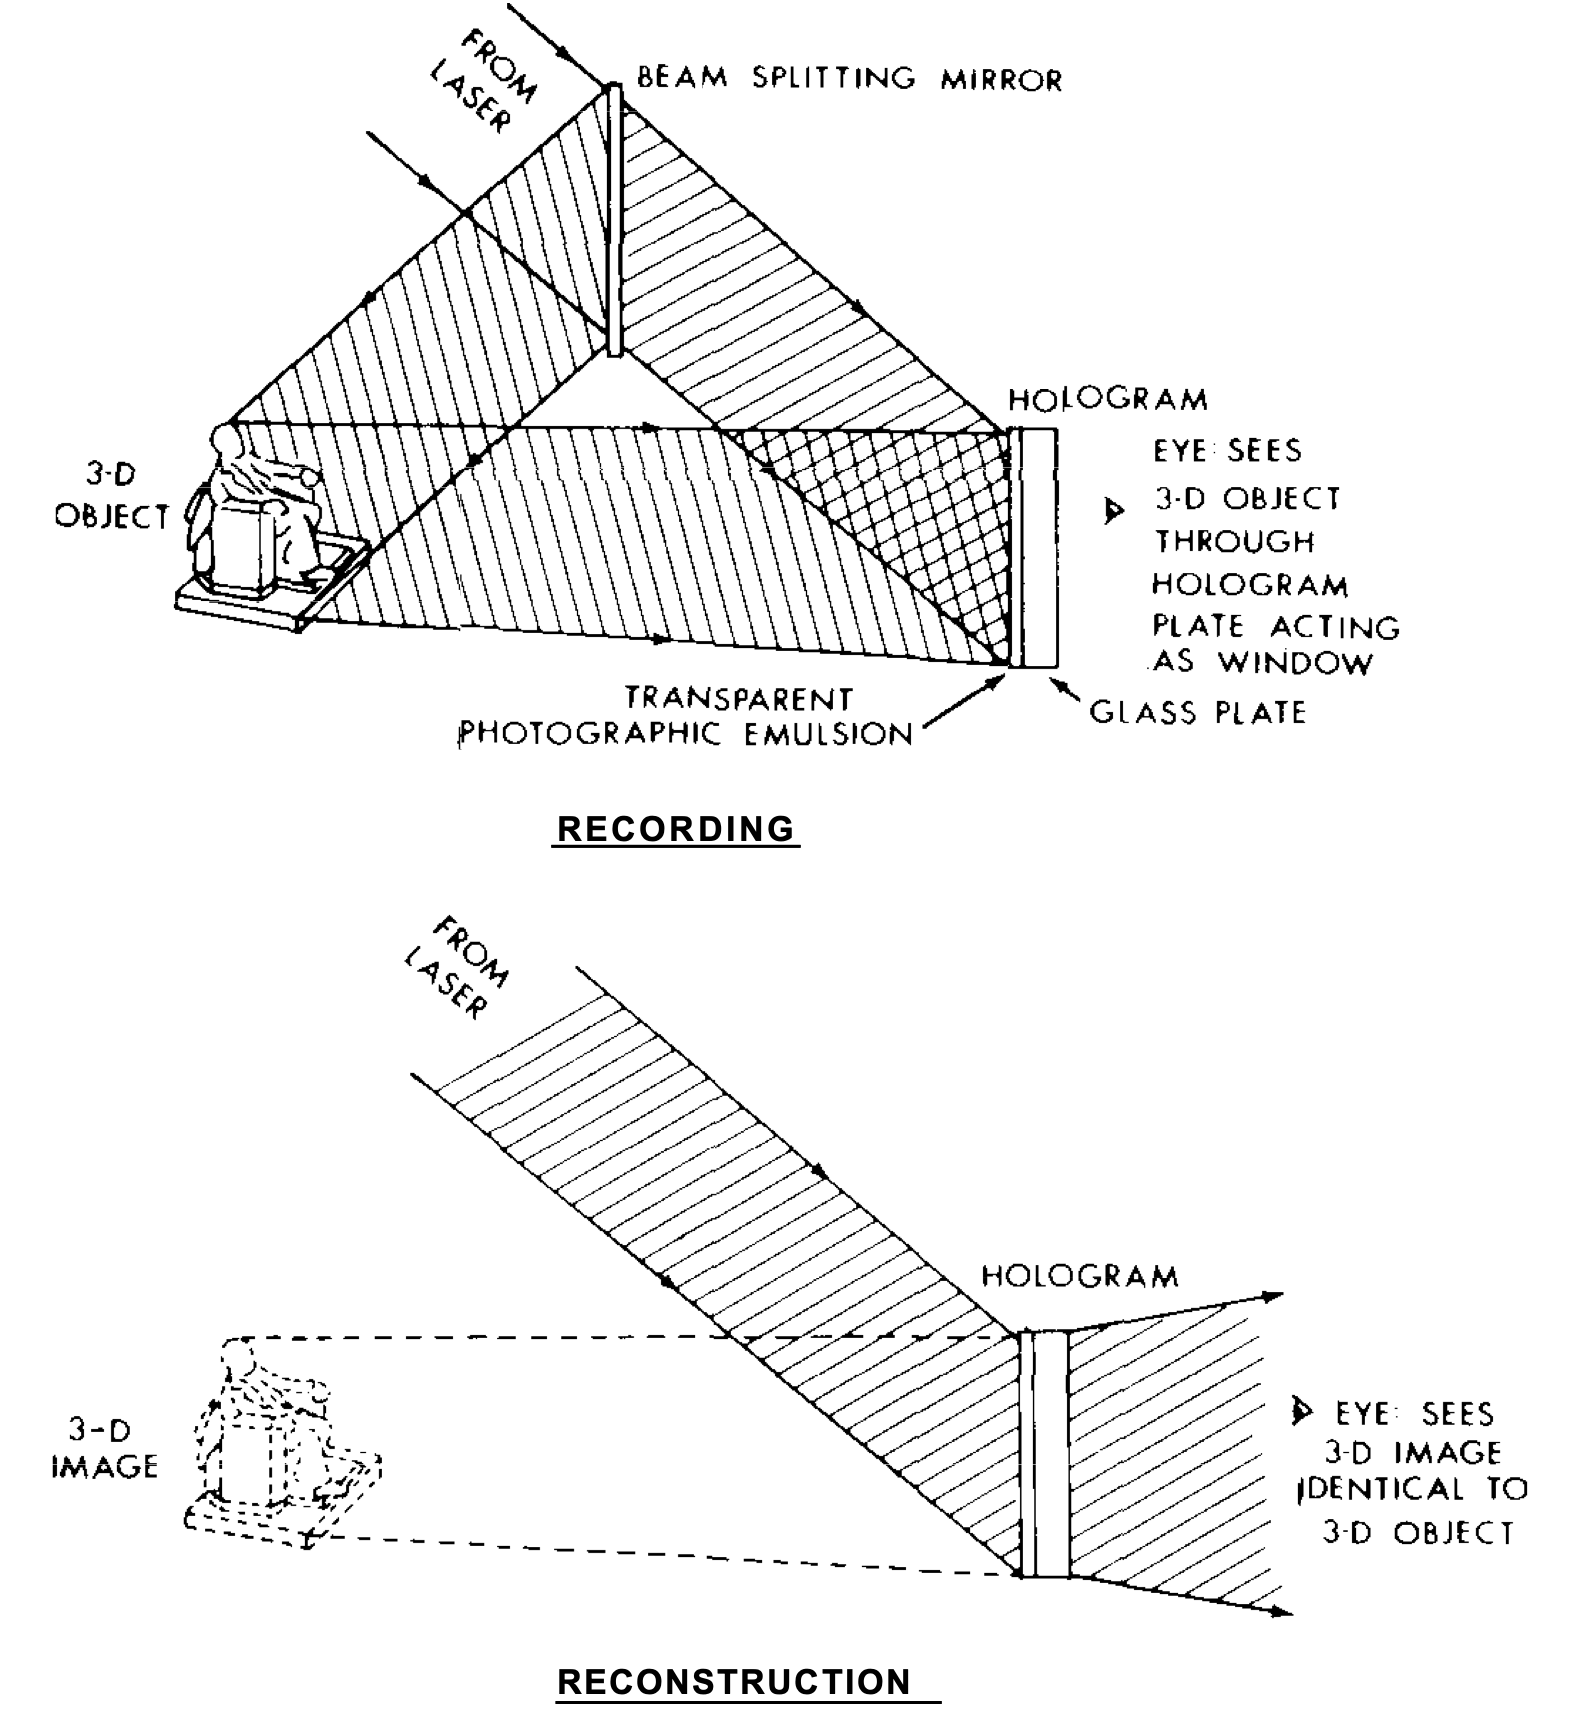
\includegraphics[width=0.5\textwidth]{images/holography.png}
    \caption{Prinzip der Holographie: Interferenz zwischen Referenz- und Objektstrahl bei einem Transmissionshologramm aus \cite{Gabor}.}
    \label{fig:holography}
\end{figure}

\section{Digitale Holographie}

\section{Anwendung in der Spektroskopie}

\section{Ausblick}

\printbibliography
\end{document}